
\section{Frontend Komposition} \label{sec:frontendComposition}

\subsection{Einführung in die Architektur}
\begin{figure}
    \centering
    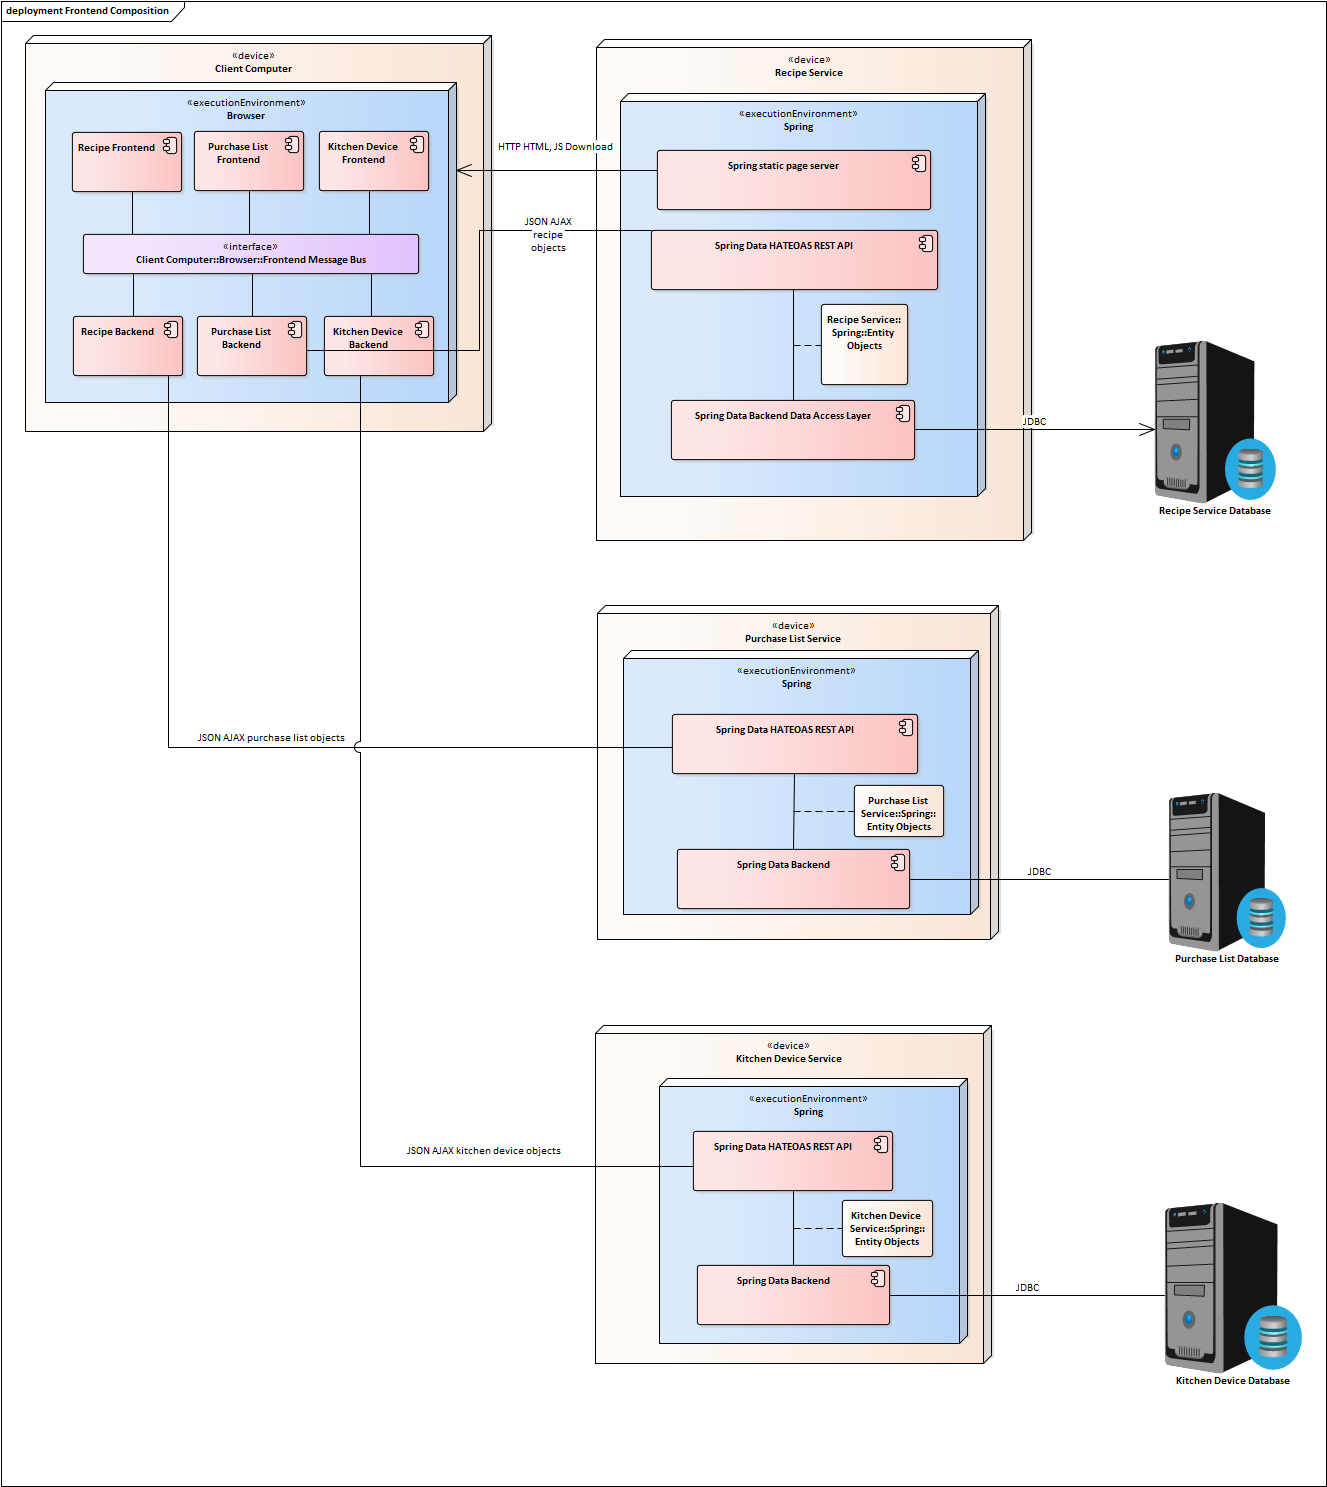
\includegraphics[width=\textwidth]{{sections/methology/assets/FrontendComposition}}
    \caption{Frontend Komposition}
    \label{fig:methology:frontendComposition:Overview}
\end{figure}

Die Frontend Komposition beschreibt das Zusammenführen \marg{Architektur} von bestehenden Webservices in einem Javascript Frontend, das Frontend führt die Daten der Services zusammen im \ac{UI}-Layer. 

Die Alternative basiert auf dem Pattern \citetitle{RichardsonFrontend} von \citeauthor{RichardsonFrontend}.

Die \marg{Implikationen} Services brauchen keinen Frontend-Layer mehr. Die Services stellen ein Web-\ac{API} bereit auf welches das Javascript-Frontend zugreifen kann.

Der Architekt erwartet die folgenden Vorteile durch die verwendete Architektur.
\begin{itemize}
    \item Die TTFB der Applikation schneller ist als bei den Alternativen
    \item Die \ac{UI} kann auch bei Nichtverfügbarkeit der Services geladen werden
    \item Die \ac{UI} kann den Ladefehler anzeigen
\end{itemize}

Es wird erwartet, dass die nachfolgenden Risiken bei der Implementierung der Alternative auftreten können.
\begin{itemize}
    \item Alle Services müssen offen ans Internet gelegt werden
\end{itemize}

\subsection{Implementation der Architektur}

\begin{figure}
    \centering
    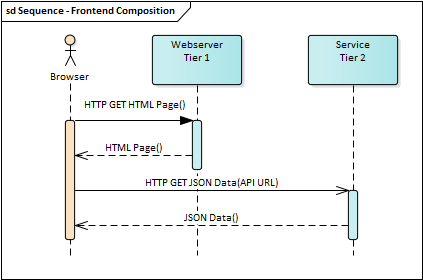
\includegraphics[width=\textwidth]{sections/methology/assets/SequenceFrontendComposition}
    \caption{Interaktion bei Frontend Komposition}
    \label{fig:sections:methology:frontendComposition:Sequence}
\end{figure}

Die Abbildung \marg{Ablauf} \ref{fig:sections:methology:frontendComposition:Sequence} zeigt das Sequenz-Diagramm der Implementierung von der Frontend Komposition in der Beispielanwendung. Der Browser ladet zuerst das statische Webdokument und rendert dieses. Sobald der Javascript geladen ist, wird ein asynchroner RESTful HTTP Request an den Service gesendet um die Daten der Ansicht zu laden. Sobald die Daten angekommen sind, werden diese ins Frontend weitergereicht und durch das Frontend angezeigt.

\begin{figure}
    \centering
\begin{lstlisting}
 return matchPath(request).map(path -> {
    LOGGER.info("Path {} was requested", path);
    model.addAttribute(TARGET_SITE_KEY, "http://localhost:9603/controller/kitchenDevice/" + path);
    model.addAttribute(TARGET_ELEMENT_KEY, path.endsWith("edit") ? "form" : "table");
    return "portal/frameHolder";
});
\end{lstlisting}
    \caption{PortalCompositionController.java, die Funktion zum Komponieren von Seiten}
    \label{fig:portalComposition:GETComposition}
\end{figure}

Währenddem \marg{Implementation} in den vorherigen Kapitel von Frontend als Webserver vorgeschaltet vor den Applikationsserver die Rede war, wird als Frontent in diesem Kapitel eine selbständige Browserapplikation genannt, die wiederum in ein Frontend und ein Backend aufgeteilt ist. Diese \ac{UI}-Applikation im Browser sollte auch ein sauberes Layering einhalten.

Zuunterst liegt der Backend-Layer, der die Datenbereitstellung für das UI übernimmt. In der Mitte kann ein Event-Bus eingerichtet werden, damit die Frontends mit dem Backend kommunizieren können. \cite{Söderlund2017}

In meiner Applikation habe ich die Backends und die Frontends umgesetzt. Diese können miteinander kommunizieren. Der Event-Bus wurde nicht mehr umgesetzt als Teil der Projektarbeit.

\subsection{Resultate aus der Programmierung der Alternative}
Die Chancen in der Frontend Komposition \marg{Chancen} sieht der Architekt in der Integration von Services verschiedener APIs. 

Die \marg{Risiken} Risiken bestehen in der gemeinsamen Verantwortung und Zuständigkeit verschiedener Teams auf einen gemeinsamen Source-Code für das Frontend. Der Code wird von verschiedenen Entwicklungsteams bearbeitet und hat keinen Eigentümer der die Verantwortung über den Code des Frontends trägt.  

\subsection{Diskussion der Alternative}

Die Implementierung zeigt die Machbarkeit von einer Frontend Integration auf. Es wurde im Zuge dieser Arbeit einen Prototyp erstellt und getestet. 

Innerhalb der vorgegeben Projektdauer konnten nicht alle Features eines Microfrontends umgesetzt werden. Der Architekt hat die nachfolgenden Features nicht umgesetzt und könnten in einer Nachfolgearbeit weitergeführt werden:

\begin{itemize}
    \item Die Trennung verschiedener Javascript-Frameworks innerhalb einers HTML-Dokumentes.
    \item Der Einsatz eines Event-Bus für die Kommunkation zwischen den Framework-Impementationen
    \item Das späte Nachladen der Frontend-Komponenten nach dem Aufbau der Website 
\end{itemize}

Der \marg{Ausblick} Architekt sieht folgende weiterführende Arbeiten:
\begin{description}
    \item[GraphQL] Ein Ansatz für Frontend zu Backend Kommunikation um die Bandbreite zu reduzieren \footnote{https://graphql.org/}
    \item[Single SPA] Dieses Projekt separiert verschiedene Frontend-Frameworks voneinander. Es erlaubt zum Beispiel eine Koexistenz von Angular und React Komponenten in der gleichen HTML Seite. \footnote{https://github.com/CanopyTax/single-spa}
    \item[Shared Event Bus] Erlaubt die Kommunikation verschiedener getrennter (siehe Single SPA) Frontend-Komponenten auf der HTML Seite.  \footnote{https://github.com/chrisdavies/eev}
\end{description}